\documentclass{beamer}

% Theme configuration
\usetheme{Madrid}
\usecolortheme{whale}

% Packages
\usepackage[utf8]{inputenc}
\usepackage{amsmath}
\usepackage{graphicx}
\usepackage{booktabs}
\usepackage{algorithm}
\usepackage{algpseudocode}

% Title Page Information
\title[Quizum]{Quizum: AI-powered Video Summarization and Quiz Generator Website}
\subtitle{Specialized Project Report}
\author[N.B. Nguyen \& D.H.T. Hung]{
    Student: Nguyen Binh Nguyen - 2252545 \\
    Student: Do Hoang Thai Hung - 2052506
}
\institute[HCMUT]{
    Supervisor: Assoc. Prof. Quan Thanh Tho, Ph.D. \\
    Vietnam National University, Ho Chi Minh City \\
    Ho Chi Minh City University of Technology
}
\date{December 2025}

\begin{document}

% Slide 1: Title
\begin{frame}
    \titlepage
    \end{frame}

% Slide 2: Table of Contents
\begin{frame}{Table of Contents}
    \tableofcontents
\end{frame}

% --- SECTION 1: INTRODUCTION ---
\section{Introduction \& Motivation}

\begin{frame}{Motivation}
    \begin{itemize}
        \item \textbf{Context:} Students and self-learners face the challenge of managing and understanding large volumes of video lectures and educational content.
        \item \textbf{Current Approaches:} Manual note-taking, passive video watching, and traditional learning tools provide limited assistance.
        \item \textbf{Limitations:}
            \begin{itemize}
                \item \textbf{Time-Consuming:} Processing lengthy lecture recordings requires significant manual effort.
                \item \textbf{Inefficient Revision:} 72\% of students struggle to revise effectively using long recorded lectures (Online Learning Consortium).
                \item \textbf{Lack of Interactive Tools:} 67\% of instructors believe students need structured summaries and interactive reinforcement tools (EDUCAUSE Review).
            \end{itemize}
    \end{itemize}
\end{frame}

\begin{frame}{Project Goals}
    To design an intelligent web-based platform (\textbf{Quizum}) that transforms educational video lectures into structured learning materials:
    \begin{block}{Key Objectives}
        \begin{enumerate}
            \item \textbf{Automatic Transcription:} Use Whisper AI to convert speech to text with timestamp segments.
            \item \textbf{AI-Powered Summarization:} Generate concise summaries using fine-tuned PEGASUS model.
            \item \textbf{Quiz Generation:} Create self-assessment quizzes using Flan-T5 for interactive learning.
            \item \textbf{Improve Learning Efficiency:} Enhance study efficiency, learner engagement, and knowledge retention.
        \end{enumerate}
    \end{block}
\end{frame}

% --- SECTION 2: RELATED WORK ---
\section{Related Work}

\begin{frame}{Related Work: VideoKen}
    \textbf{VideoKen} - Interactive video learning platform for enterprise L\&D
    
    \begin{columns}
        \column{0.5\textwidth}
        \textbf{Key Features:}
        \begin{itemize}
            \item \textbf{Auto-generated chapters:} AI analyzes visual/audio to segment videos
            \item \textbf{Phrase clouds:} Navigate to specific topics instantly
            \item \textbf{Deep search:} Search spoken words across video library
            \item \textbf{In-video quizzes:} Manual embedding of assessments
        \end{itemize}
        
        \column{0.5\textwidth}
        \textbf{Limitations:}
        \begin{itemize}
            \item Focus on navigational indexing
            \item Manual quiz creation (not automated)
            \item Enterprise-focused, not education
            \item No automated assessment generation
        \end{itemize}
    \end{columns}
\end{frame}

\begin{frame}{Related Work: Otter.ai \& Kwizie}
    \begin{columns}
        \column{0.5\textwidth}
        \textbf{Otter.ai} - Meeting transcription
        \begin{itemize}
            \item Real-time transcription
            \item Speaker identification
            \item Executive summaries
            \item Keyword extraction
            \item \textcolor{red}{Limitation:} No quiz generation
        \end{itemize}
        
        \column{0.5\textwidth}
        \textbf{Kwizie} - Gamified quiz platform
        \begin{itemize}
            \item AI quiz generation from videos
            \item Multiplayer game format
            \item Microlearning approach
            \item LLM-powered MCQ creation
            \item \textcolor{red}{Limitation:} No summarization
        \end{itemize}
    \end{columns}
    
    \vspace{0.3cm}
    \textbf{Quizum's Advantage:} Integrates transcription + summarization + quiz generation in one cohesive workflow
\end{frame}

\begin{frame}{Related Work: Comparison}
    \begin{table}
        \centering
        \small
        \begin{tabular}{lccc}
            \toprule
            \textbf{Feature} & \textbf{VideoKen} & \textbf{Otter.ai} & \textbf{Kwizie} \\
            \midrule
            Speech-to-Text & Yes & \textbf{Yes} & Yes \\
            Auto Summarization & Phrase clouds & \textbf{Yes} & No \\
            Auto Quiz Gen & No & No & \textbf{Yes} \\
            Interactive Quizzes & Yes & No & \textbf{Yes} \\
            AI Chatbot/Q\&A & Search-based & Yes & No \\
            \midrule
            \textbf{Target Audience} & Enterprise & Business & Education \\
            \bottomrule
        \end{tabular}
        \caption{Comparison of related platforms}
    \end{table}
    
    \vspace{0.2cm}
    \textbf{Quizum uniquely combines:} Transcription + Summarization + Quiz Generation + Interactive Learning
\end{frame}

% --- SECTION 3: SYSTEM REQUIREMENTS ---
\section{System Requirements \& Design}

\begin{frame}{Stakeholders \& Their Needs}
    \begin{itemize}
        \item \textbf{Students (Primary Users):}
            \begin{itemize}
                \item Time-saving platform for quick revision
                \item Accurate, concise summaries
                \item Accessibility across devices
            \end{itemize}
        
        \item \textbf{Educators:}
            \begin{itemize}
                \item Insights into student engagement
                \item Identify knowledge gaps
                \item Ensure information accuracy
            \end{itemize}
        
        \item \textbf{Developers:}
            \begin{itemize}
                \item Scalable, performant system
                \item Clear requirements and feedback loops
                \item Seamless integration capabilities
            \end{itemize}
        
        \item \textbf{Content Creators:}
            \begin{itemize}
                \item Intellectual property protection
                \item Increased lecture impact and accessibility
            \end{itemize}
    \end{itemize}
\end{frame}

\begin{frame}{System Benefits}
    \textbf{Key Benefits for All Stakeholders:}
    
    \begin{columns}
        \column{0.5\textwidth}
        \textbf{For Learners:}
        \begin{itemize}
            \item \textbf{Time savings:} Quick revision without rewatching
            \item \textbf{Better retention:} 25\% improvement with summaries + quizzes
            \item \textbf{Personalized learning:} Focus on weak areas
            \item \textbf{Interactive engagement:} Active vs passive learning
        \end{itemize}
        
        \column{0.5\textwidth}
        \textbf{For Educators:}
        \begin{itemize}
            \item Track student interaction patterns
            \item Identify knowledge gaps
            \item Enhanced teaching effectiveness
            \item Reduced manual quiz creation
        \end{itemize}
    \end{columns}
    
    \vspace{0.3cm}
    \textbf{Institutional Value:} Improved student performance, innovation in digital learning, scalable platform
\end{frame}

\begin{frame}{Functional Requirements}
    \begin{enumerate}
        \item \textbf{Video Input \& Preprocessing:}
            \begin{itemize}
                \item Accept URL (YouTube) or file upload (MP4, AVI, MOV; max 500MB)
                \item Transcribe with Whisper (85\%+ accuracy on clear audio)
                \item Preserve timestamps for segment linking
            \end{itemize}
        
        \item \textbf{Summarization Module:}
            \begin{itemize}
                \item Generate extractive/abstractive summaries (10-20\% of original)
                \item Extract main topics, key points, conclusions
                \item Output: Plain text, bullets, or PDF with timestamps
            \end{itemize}
        
        \item \textbf{Quiz Generation:}
            \begin{itemize}
                \item Auto-generate 5-15 questions per video
                \item Types: MCQ (4 options), true/false, fill-in-blank
                \item Include correct answer + explanation
            \end{itemize}
    \end{enumerate}
\end{frame}

\begin{frame}{Non-Functional Requirements}
    \textbf{Performance:}
    \begin{itemize}
        \item Process 10-min video in under 2 minutes (transcription + summarization + quiz)
        \item Handle videos up to 2 hours without crashing
        \item \textbf{Accuracy targets:}
            \begin{itemize}
                \item Transcription: 85\%+ (WER metric)
                \item Summary coherence: 80\%+ (ROUGE score)
                \item Quiz relevance: 90\%+ (human-evaluated)
            \end{itemize}
    \end{itemize}
    
    \textbf{Usability:}
    \begin{itemize}
        \item No technical expertise required
        \item Tooltips, tutorials, demo videos
        \item Default English, with localization options
    \end{itemize}
    
    \textbf{Security \& Reliability:}
    \begin{itemize}
        \item User data protection and privacy
        \item 99\% uptime target
    \end{itemize}
\end{frame}

\begin{frame}{Use Case Overview}

    \begin{columns}
        \column{0.48\textwidth}
        \textbf{UC-01: Upload Video}
        \begin{itemize}
            \item User uploads video/link
            \item System validates format
            \item Queues for transcription
        \end{itemize}
        
        \vspace{0.5em}
        
        \textbf{UC-02: Summarize Video}
        \begin{itemize}
            \item Retrieves transcript
            \item Generates summary
            \item Displays to user
        \end{itemize}
        
        \vspace{0.5em}
        
        \textbf{UC-03: Generate Quiz}
        \begin{itemize}
            \item Analyzes transcript
            \item Creates questions
            \item Stores for practice
        \end{itemize}
        
        \column{0.48\textwidth}
        \textbf{UC-04: Take Quiz}
        \begin{itemize}
            \item User answers questions
            \item System evaluates
            \item Provides feedback
        \end{itemize}
        
        \vspace{0.5em}
        
        \textbf{UC-05: Download/Export Results}
        \begin{itemize}
            \item User selects format
            \item System generates file
            \item User downloads content
        \end{itemize}
    \end{columns}
\end{frame}



% --- SECTION 4: SYSTEM ARCHITECTURE ---
\section{System Architecture}

\begin{frame}{System Overview}
    The system implements a modern, decoupled client-server architecture with three primary layers:
    
    \begin{enumerate}
        \item \textbf{Frontend Layer:}
            \begin{itemize}
                \item Next.js (React-based)
                \item Server-side rendering (SSR)
                \item Real-time video playback
            \end{itemize}
        \item \textbf{Backend Layer:}
            \begin{itemize}
                \item Node.js + Express
                \item RESTful API
                \item Request validation
            \end{itemize}
        \item \textbf{Worker Layer:}
            \begin{itemize}
                \item BullMQ + Redis queue
                \item Async AI processing
            \end{itemize}
    \end{enumerate}
\end{frame}

\begin{frame}{System Architecture Diagram}
    \begin{figure}
        \centering
        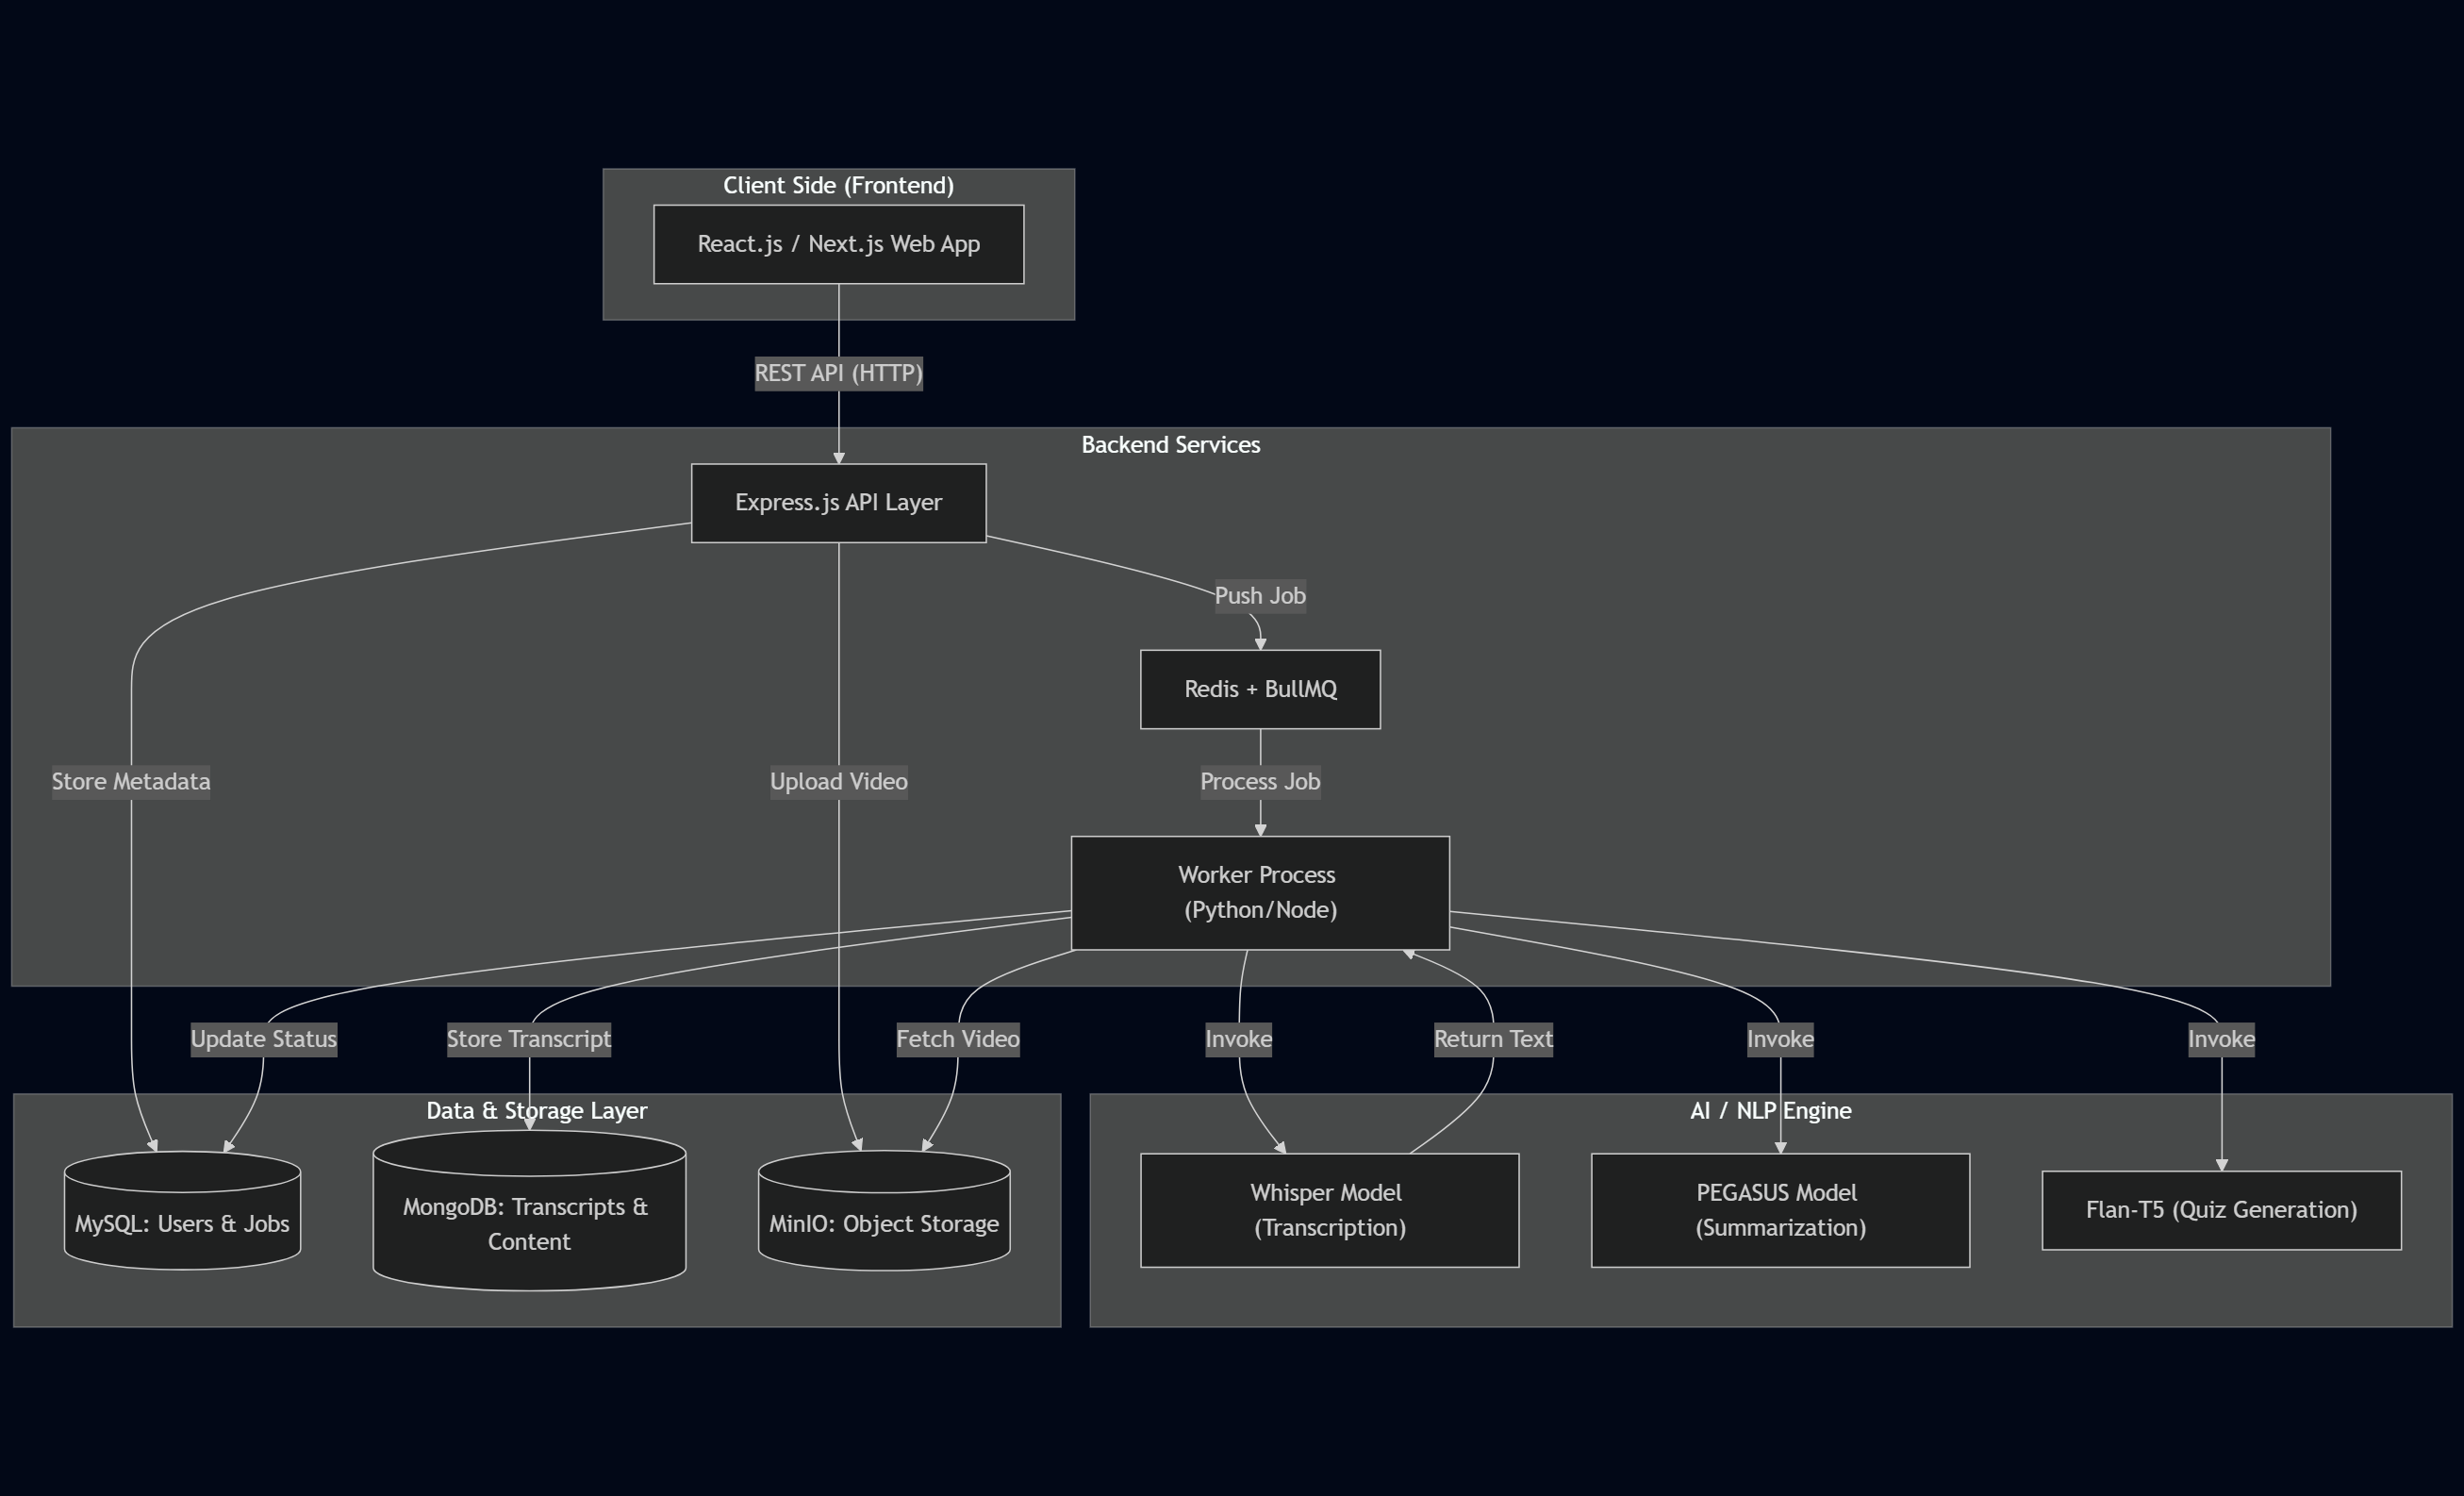
\includegraphics[width=0.8\textwidth]{images/1. System_Architecture_Diagram.png}
        \caption{System Architecture Diagram}
    \end{figure}
\end{frame}

\begin{frame}{AI Processing Pipeline}
    The worker service orchestrates three AI models for content processing:
    
    \begin{enumerate}
        \item \textbf{Whisper (Speech-to-Text):}
            \begin{itemize}
                \item Robust transcription with timestamp segments
                \item Multiple model sizes (Tiny to Large)
                \item Selected: Whisper Small (optimal balance)
            \end{itemize}
        
        \item \textbf{PEGASUS (Summarization):}
            \begin{itemize}
                \item Fine-tuned on SAMSum dataset (14,732 conversations)
                \item Abstractive summarization for dialogue
                \item Generates concise, coherent summaries
            \end{itemize}
        
        \item \textbf{Flan-T5 (Quiz Generation):}
            \begin{itemize}
                \item Instruction-tuned model
                \item Generates multiple-choice questions
                \item Links questions to transcript segments
            \end{itemize}
    \end{enumerate}
\end{frame}

\begin{frame}{Data Storage Strategy}
    The system uses a \textbf{polyglot persistence} approach to handle different data types efficiently:
    
    \begin{itemize}
        \item \textbf{MySQL (Relational):}
            \begin{itemize}
                \item Job tracking and status management
                \item User accounts and authentication
                \item Quiz metadata and attempts
                \item Structured queries and consistency
            \end{itemize}
        
        \item \textbf{MongoDB (Document):}
            \begin{itemize}
                \item Full transcripts with segments
                \item Flexible schema for varying content
                \item Efficient for large text documents
            \end{itemize}
        
        \item \textbf{MinIO (Object Storage):}
            \begin{itemize}
                \item S3-compatible storage
                \item Video and audio assets
                \item Staging for future AWS S3 migration
            \end{itemize}
    \end{itemize}
\end{frame}

\begin{frame}{Database Schema: MySQL}

    \begin{columns}
        \column{0.5\textwidth}
        \textbf{Core Tables:}
        \begin{itemize}
            \item \textbf{jobs:} UUID, status (ENUM), payload (JSON), result (JSON)
            \item \textbf{videos:} id, owner\_id, storage\_key, status
            \item \textbf{users:} email, password\_hash, role
        \end{itemize}
        
        \column{0.5\textwidth}
        \textbf{Assessment Tables:}
        \begin{itemize}
            \item \textbf{quizzes:} video\_id (FK), type
            \item \textbf{questions:} text, options (JSON), answer, source\_segments
            \item \textbf{quiz\_attempts:} score, details (JSON)
        \end{itemize}
    \end{columns}
    
    \vspace{0.3cm}
    \textbf{Key Features:}
    \begin{itemize}
        \item Foreign key relationships for data integrity
        \item JSON columns for flexible data (payload, options, details)
        \item Status tracking with ENUM types for consistency
        \item Source\_segments link questions to video timestamps
    \end{itemize}
\end{frame}

\begin{frame}{MySQL Database Schema}
    \begin{figure}
        \centering
        \includegraphics[width=0.85\textwidth]{images/mysql_schema.png}
        \caption{MySQL Database Entity Relationship Diagram}
    \end{figure}
\end{frame}

\begin{frame}{MongoDB \& Data Flow}

    \begin{columns}
        \column{0.5\textwidth}
        \textbf{Transcript Collection:}
        \begin{itemize}
            \item \textbf{videoId:} Link to MySQL job
            \item \textbf{fullText:} Complete transcription
            \item \textbf{segments:} Array of \{start, end, text\}
        \end{itemize}
        
        \vspace{0.2cm}
        \textbf{Why MongoDB?}
        \begin{itemize}
            \item Flexible schema for varying content
            \item Efficient for large text documents
            \item Supports full-text search
        \end{itemize}
        
        \column{0.5\textwidth}
        \textbf{Data Flow:}
        \begin{enumerate}
            \item Upload → Redis queue (volatile)
            \item Worker processes job
            \item Save transcript to MongoDB
            \item Update job status in MySQL
        \end{enumerate}
        
        \vspace{0.2cm}
        \textbf{Hybrid Strategy Benefits:}
        \begin{itemize}
            \item Fast structured queries (MySQL)
            \item Efficient content retrieval (MongoDB)
            \item Optimized for both use cases
        \end{itemize}
    \end{columns}
\end{frame}

% --- SECTION 5: EXPERIMENTAL RESULTS ---
\section{Experimental Results}

\begin{frame}{Whisper Model Evaluation}
    \begin{columns}
        \column{0.5\textwidth}
        \textbf{Setup:}
        \begin{itemize}
            \item \textbf{Test Audio:} 30-minute Yale lecture (PSYC 110)
            \item \textbf{Hardware:} Tesla T4 GPU (16GB), 12.7GB RAM
            \item \textbf{Platform:} Google Colab
            \item \textbf{Models Tested:}
                \begin{itemize}
                    \item Tiny (190MB)
                    \item Base (285MB)
                    \item Small (1094MB)
                    \item Medium (3309MB)
                    \item Large (4649MB)
                \end{itemize}
        \end{itemize}
        
        \column{0.5\textwidth}
        \textbf{Metrics:}
        \begin{itemize}
            \item \textbf{WER:} Word Error Rate
            \item \textbf{CER:} Character Error Rate
            \item \textbf{Speed:} Inference time (seconds)
            \item \textbf{Memory:} Model size
        \end{itemize}
    \end{columns}
\end{frame}

\begin{frame}{Results: Accuracy vs Speed Trade-off}
    Whisper Small provides the best balance of accuracy, speed, and memory usage.
    
    \begin{table}
        \centering
        \small
        \begin{tabular}{lccc}
            \toprule
            \textbf{Model} & \textbf{WER (\%)} & \textbf{CER (\%)} & \textbf{Speed (s)} \\
            \midrule
            Tiny & 20.02 & 16.90 & \textbf{49.5} \\
            Base & 19.22 & 16.50 & 61.6 \\
            \textbf{Small} & \textbf{18.68} & \textbf{16.47} & \textbf{114.1} \\
            Medium & \textbf{18.27} & \textbf{16.36} & 201.7 \\
            Large & 19.58 & 17.69 & 279.2 \\
            \bottomrule
        \end{tabular}
        \caption{Whisper Model Performance Comparison}
    \end{table}
    \vspace{0.2cm}
    \textbf{Key Finding:} Whisper Small selected as optimal model - only 0.4\% WER difference from Medium, but \textbf{43\% faster} (114s vs 201s).
    
\end{frame}

\begin{frame}{Results: Accuracy vs Speed Trade-off (Chart)}
    \begin{center}
        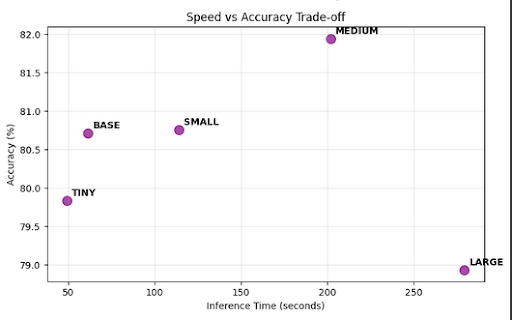
\includegraphics[width=0.8\textwidth]{images/1 chart.png}
    \end{center}
\end{frame}

\begin{frame}{PEGASUS Summarization Results}
    \begin{columns}
        \column{0.5\textwidth}
        \textbf{Training Details:}
        \begin{itemize}
            \item \textbf{Dataset:} SAMSum (14,732 conversations)
            \item \textbf{Model:} Google PEGASUS
            \item \textbf{Task:} Dialogue summarization
            \item \textbf{Approach:} Fine-tuning for conversational text
        \end{itemize}
        
        \column{0.5\textwidth}
        \textbf{Performance:}
        \begin{itemize}
            \item Generates concise summaries
            \item Maintains coherence
            \item Captures key dialogue points
            \item Optimized for lecture transcripts
        \end{itemize}
    \end{columns}

\end{frame}

\begin{frame}{PEGASUS Summarization Performance}
    \begin{figure}
        \centering
        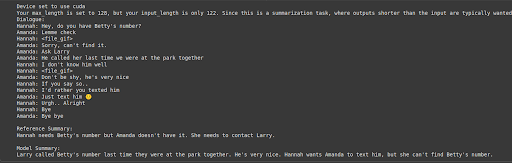
\includegraphics[width=0.8\textwidth]{images/result1.png}
        \caption{PEGASUS training and validation performance}
    \end{figure}
\end{frame}

\begin{frame}{Flan-T5 Quiz Generation Experiments}
    \begin{columns}
        \column{0.5\textwidth}
        \textbf{Experimental Setup:}
        \begin{itemize}
            \item \textbf{Model:} google/flan-t5-base
            \item \textbf{Method:} PEFT (LoRA) for efficient fine-tuning
            \item \textbf{Dataset:} RACE (Reading Comprehension from Examinations)
            \item \textbf{Goal:} Generate valid MCQ with Article, Question, Options, and Answer
        \end{itemize}
        
        \column{0.5\textwidth}
        \textbf{Zero-Shot Baseline:}
        \begin{itemize}
            \item Initial performance was poor
            \item Generated malformed, repetitive outputs
            \item Failed to follow MCQ structure
        \end{itemize}
    \end{columns}
    
    \vspace{0.2cm}
    \begin{center}
        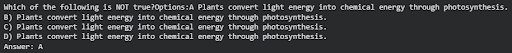
\includegraphics[width=0.8\textwidth]{images/flan_zero.png}
    \end{center}
\end{frame}

\begin{frame}{Flan-T5 Fine-Tuning Results}
    \textbf{Training Outcome (1 Epoch, $\approx$62k examples):}
    \begin{itemize}
        \item \textbf{Syntactic Success:} Model successfully learned the MCQ format (generating distinct options A, B, C, D).
        \item \textbf{Semantic Challenge:} Still struggles with deep reasoning to consistently identify the \textit{correct} answer.
    \end{itemize}
    
    \begin{figure}
        \centering
        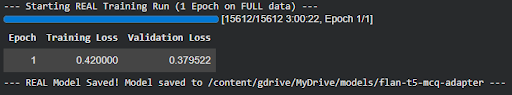
\includegraphics[width=0.85\textwidth]{images/flan_epoch.png}
        \caption{Flan-T5 generation examples after fine-tuning}
    \end{figure}
\end{frame}

% --- SECTION 6: BACKEND TESTING ---
\section{Backend Implementation Testing}

\begin{frame}{Backend Test: Video Upload API}
    \textbf{Testing POST /api/upload}
    \begin{center}
        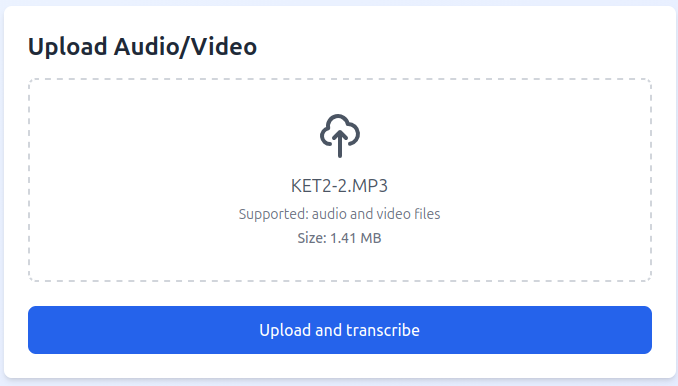
\includegraphics[width=0.9\textwidth]{images/upload.png}
    \end{center}
    \vspace{0.2cm}
    \small Validates file upload handling, MinIO storage integration, and initial job creation in MySQL.
\end{frame}

\begin{frame}{Backend Test: Job Management}
    \begin{columns}
        \column{0.5\textwidth}
        \textbf{Job Listing (GET /api/jobs)}
        \centering
        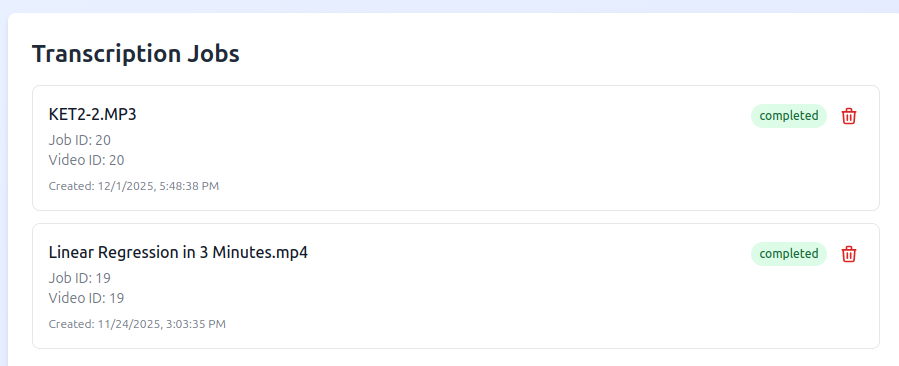
\includegraphics[width=\linewidth]{images/list.png}
        
        \column{0.5\textwidth}
        \textbf{Job Deletion (DELETE)}
        \centering
        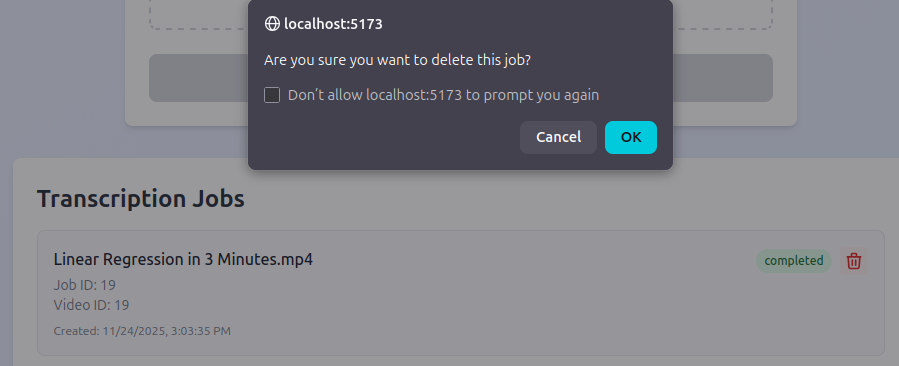
\includegraphics[width=\linewidth]{images/delete.png}
    \end{columns}
    \vspace{0.3cm}
    \small Verifies pagination metadata and cascading deletion of job records and transcripts.
\end{frame}

\begin{frame}{Backend Test: Transcript Retrieval}
    \textbf{Testing GET /api/transcripts/:videoId}
    \begin{center}
        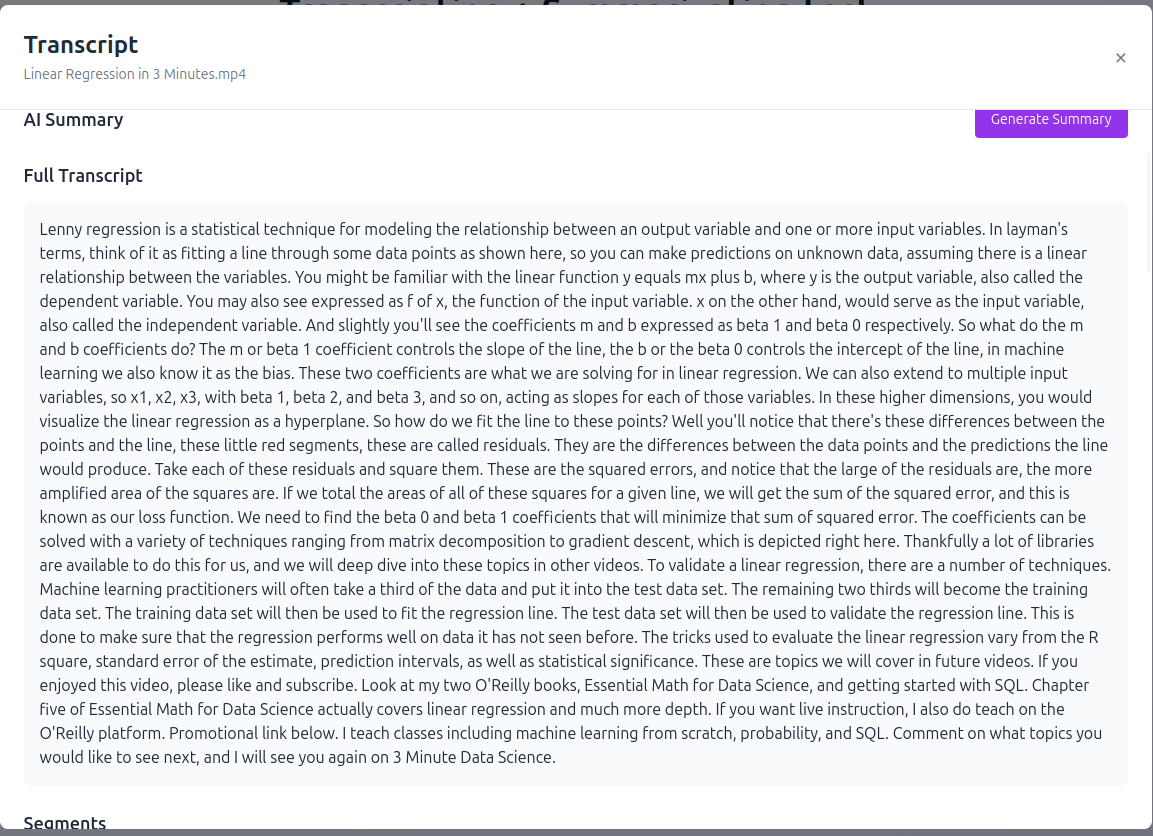
\includegraphics[width=0.85\textwidth]{images/transcript.png}
    \end{center}
    \vspace{0.2cm}
    \small Confirms successful retrieval of full transcript documents including timestamped segments from MongoDB.
\end{frame}

\begin{frame}{Backend Test: Job Details \& Playback}
    \textbf{Testing GET /api/jobs/:jobId}
    \begin{center}
        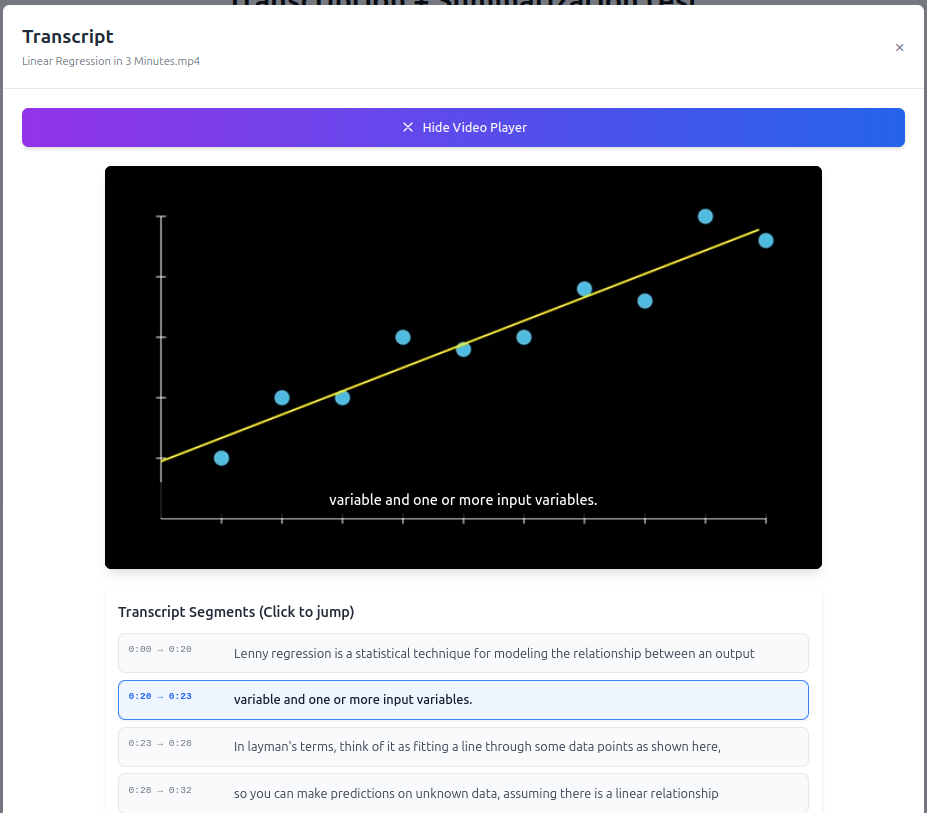
\includegraphics[width=0.8\textwidth]{images/player.png}
    \end{center}
    \vspace{0.2cm}
    \small Generates presigned URL for secure playback and retrieves comprehensive job metadata.
\end{frame}

\begin{frame}{Backend Test: Transcript Retrieval}
    \textbf{Testing GET /api/transcripts/:videoId}
    \begin{center}
        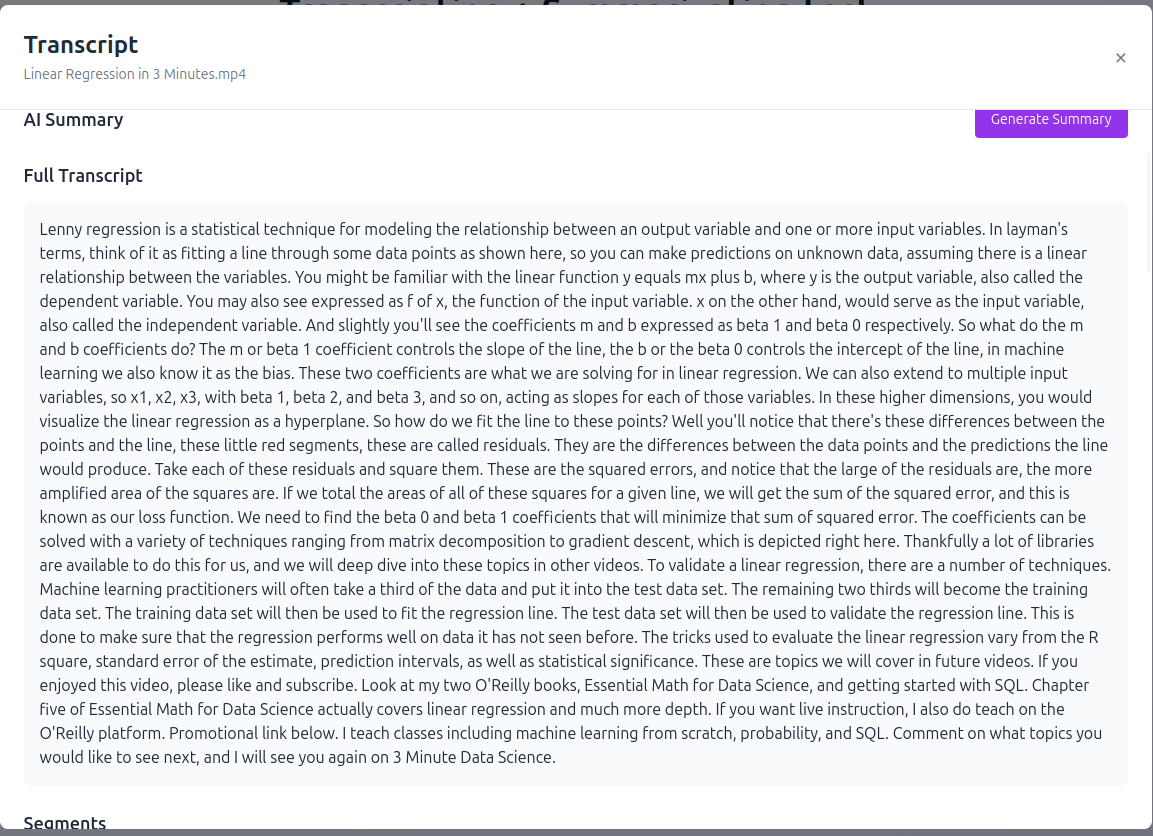
\includegraphics[width=0.85\textwidth]{images/transcript.png}
    \end{center}
    \vspace{0.2cm}
    \small Confirms successful retrieval of full transcript documents including timestamped segments from MongoDB.
\end{frame}

\begin{frame}{Backend Test: Summarization Trigger}
    \textbf{Testing POST /api/transcripts/:videoId/summarize}
    \begin{center}
        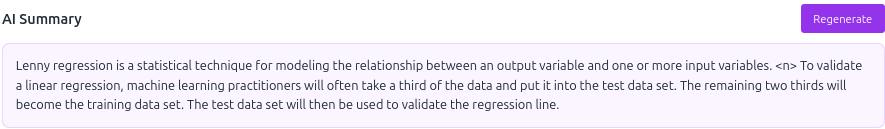
\includegraphics[width=0.85\textwidth]{images/summarize.png}
    \end{center}
    \vspace{0.2cm}
    \small Triggers the PEGASUS model to generate an abstractive summary of the transcript.
\end{frame}

% --- SECTION 6: CONCLUSION ---
\section{Conclusion \& Future Work}

\begin{frame}{Conclusion}
    \begin{enumerate}
        \item \textbf{Contribution:} Successfully implemented an end-to-end AI-powered learning platform.
        \item \textbf{Technical Achievements:} 
            \begin{itemize}
                \item Integrated Whisper (Small) for optimal transcription
                \item Fine-tuned PEGASUS on SAMSum for dialogue summarization
                \item Implemented polyglot persistence (MySQL + MongoDB + MinIO)
                \item Built async processing pipeline with BullMQ + Redis
            \end{itemize}
        \item \textbf{Impact:}
            \begin{itemize}
                \item Transforms passive video watching into active learning
                \item Reduces manual effort in study preparation
                \item Provides interactive quizzes for self-assessment
            \end{itemize}
    \end{enumerate}
\end{frame}

\begin{frame}{Future Work}

    \begin{block}{Planned Enhancements}
        \begin{itemize}
            \item \textbf{MCQ Generator model:} Upgrade to a larger model for multiple difficulty levels and high diversity.
            \item \textbf{AWS S3 Migration:} Transition from MinIO to AWS S3 for improved reliability and scalability.
            \item \textbf{Cloud Deployment:} Deploy to production environment with CI/CD pipeline.
            \item \textbf{New Features:}
                \begin{itemize}
                    \item Automatic mind-map generation from transcripts
                    \item Integrated AI chatbot for Q\&A and content guidance
                    \item Flashcard generation for reinforcement learning
                \end{itemize}
        \end{itemize}
    \end{block}
\end{frame}

\begin{frame}
    \centering
    \Huge \textbf{Q \& A} \\
    \vspace{1cm}
    \large Thank you for your attention!
\end{frame}

\end{document}